\documentclass[tikz,border=2pt]{standalone}
\usepackage{amsmath}
\usetikzlibrary{arrows.meta}
\begin{document}
% A = [[1,1],[0,1]] maps the unit circle onto an ellipse with semi-axes sigma_1 = (1+sqrt5)/2 ~ 1.618
% and sigma_2 = (sqrt5-1)/2 ~ 0.618; the unit vectors (0.526,0.851) and (-0.851,0.526) go to the semi-axes.
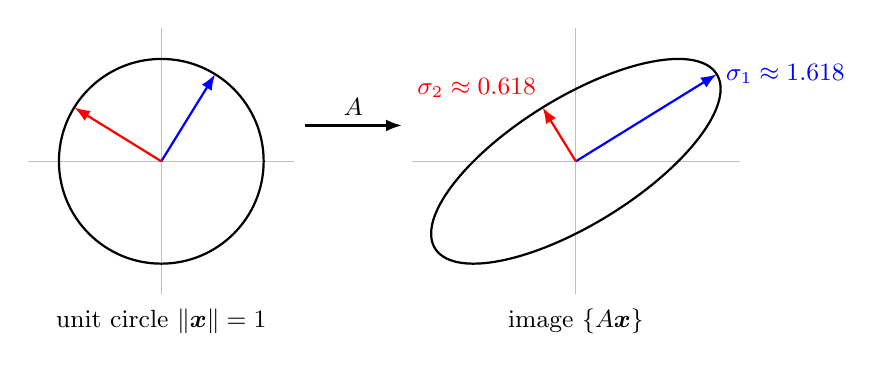
\begin{tikzpicture}[font=\small, >={Latex[length=2mm]}, x=1.3cm, y=1.3cm]
  % left: unit circle
  \draw[gray!50, thin] (-1.3,0) -- (1.3,0);
  \draw[gray!50, thin] (0,-1.3) -- (0,1.3);
  \draw[thick] (0,0) circle (1);
  \draw[->, thick, blue] (0,0) -- (0.5257,0.8507);
  \draw[->, thick, red] (0,0) -- (-0.8507,0.5257);
  \node[anchor=north] at (0,-1.35) {unit circle $\|\boldsymbol{x}\|=1$};
  % map
  \draw[->, thick] (1.4,0.35) -- (2.35,0.35) node[midway, above] {$A$};
  % right: image ellipse
  \begin{scope}[shift={(4.05,0)}]
    \draw[gray!50, thin] (-1.6,0) -- (1.6,0);
    \draw[gray!50, thin] (0,-1.3) -- (0,1.3);
    \draw[thick] plot[domain=0:360, samples=120, smooth] ({cos(\x)+sin(\x)},{sin(\x)});
    \draw[->, thick, blue] (0,0) -- (1.3764,0.8507) node[right, inner sep=3pt] {$\sigma_1\approx1.618$};
    \draw[->, thick, red] (0,0) -- (-0.3249,0.5257) node[left, inner sep=2pt, yshift=7pt] {$\sigma_2\approx0.618$};
    \node[anchor=north] at (0,-1.35) {image $\{A\boldsymbol{x}\}$};
  \end{scope}
\end{tikzpicture}
\end{document}
